%!TEX root = ../thesis.tex
%*******************************************************************************
%*********************************** First Chapter *****************************
%*******************************************************************************

\chapter{Data-driven science}  %Title of the First Chapter
\label{chap:intro_stat}
\ifpdf
    \graphicspath{{Chapter1/Figs/Raster/}{Chapter1/Figs/PDF/}{Chapter1/Figs/}}
\else
    \graphicspath{{Chapter1/Figs/Vector/}{Chapter1/Figs/}}
\fi

\victor{This is a example of comment}

\cecile{This is a example of comment}

\isabelle{This is a example of comment}

\david{This is a example of comment}

\topic{This is a example of topic}
\content{This is a example of content}


\topic{Simulations combined with machine learning make possible to extract knowledge even in highly complex and stochastic process like High Energy Physics}

\content{Objectif : Improving the precision of parameter estimation in a special case of the inverse problem in the presence of systematic effect.}






\section{LHC experiments} % (fold)
\label{sec:lhc_experiments}

\topic{C'est très complexe mais on a pas besoin de toute cette complexité pour saisir le problème.}






\subsection{Counting problem} % (fold)
\label{sub:counting_problem}

The system producing the data studied in this analysis is the famous Large Hardon Collider (LHC).
Without getting into the details a particle collider is a machine accelerating small bricks of matter, protons in this case, in opposite direction to smash them against each others.
The resulting collision produces high energy particles whose properties are captured by the various measurement apparatus which is reduced here for simplicity to a "giant camera".

\begin{figure}[htb]
    \centering
    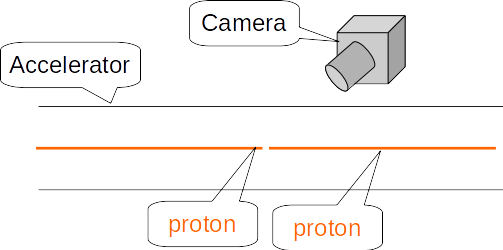
\includegraphics[width=0.8\linewidth]{particle_collider_0}
    \caption{Very simple particle collider}
    \label{fig:particle_collider_0}
\end{figure}


These collisions can be classified into 2 kinds :
\begin{itemize}
	\item the soft collisions when the protons "missed" each other and does not produce high energy particles
	\item the hard collisions when the protons smashed on each other and produces many particles
\end{itemize}

\begin{figure}[htb]
  \centering
  \begin{subfigure}[t]{0.49\linewidth}
    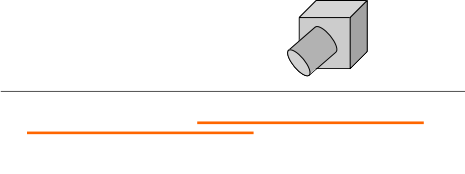
\includegraphics[width=\linewidth]{particle_collider_soft}
    \caption{soft collision}
    \label{fig:soft_collision}
  \end{subfigure}%
  \hfill
  \begin{subfigure}[t]{0.49\linewidth}
    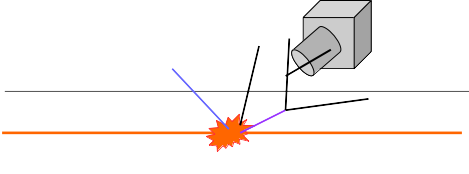
\includegraphics[width=\linewidth]{particle_collider_hard}
    \caption{hard collision}
    \label{fig:hard_collision}
  \end{subfigure}
  \caption{soft collision (left) and hard collision (right)}
  \label{fig:collision}
\end{figure}

The hard collisions, named \emph{event} in the field of High Energy Physics (HEP), are way rarer than the soft one.
The process creating the high energy particles is fundamentally stochastic.
Meaning that the nature and properties (eg. kinematics) of the produced particles are not fully predictable but follow
probability distributions whose shapes and properties are deterministics.

The vast majority of the particles created in the process are already well known.
To produce rare, therefore interesting, particles the accelerator must produce millions collisions each seconds.

The LHC is housing many experiments.
The one that is of interest in this work is a measurement of the frequency of a specific process ( H to tau tau).
Each event following this process is defined as a \emph{signal} event versus the \emph{background} events that gather all the other processes.
Leading to a counting experiment of the number of signals $s$ and the number of backgrounds $b$ to give access to the value of interest $\frac{s}{s + b}$.

In many interesting cases, including ours, the nature of the event (signal/background) are not among the possible measurement that can be made.


\content{Introduce cross section estimations / mixture coefficient inference ?}
$m$ is therefore connected to branch factor (cross section ?) of the Higgs boson which is the parameter we want to measure.
\victor{Link between cross-section, branch factor, luminosity ?}





\subsection{The model} % (fold)
\label{sub:the_model}

The theory describing particle collisions and productions is the Standard Model \needcite (SM).
The counting experiment final objective is to improve our knowledge of one of the free parameter of the SM.
In other word we are fitting the SM parameters to the data of the experiment.

The model of the experiment includes several major steps : 
\begin{enumerate}
	\item The collision
	\item The particle production from the collision
	\item Particle desintegrations into other particles and interactions between produced particles
	\item Reaction of the measurement apparatus to the particles going through it.
\end{enumerate}

Each of these steps is very complex and requires a lot of work from the community.

\victor{L'objectif est de donner un apperçu de la complexité de la chose. Sans entrer + que ça dans les détails...}
\victor{TODO : Donner un aperçu de la complexité de chaque étape en 1 ou 2 phrases.}






\section{Inference through simulation} % (fold)
\label{sec:inference_through_simulation}

\victor{Or "Inference with/using simulations" ?}

\topic{Simulations/models are useful to explain data (therefore understand the undelying process that generated the data)}


\content{Dans un monde simple tout est "facile"}
\content{Introduire le problème d'extraction d'un coefficient de mélange(lié à cross-section)}







\subsection{Classic parameter estimation} % (fold)
\label{sub:classic_parameter_estimation}

\topic{Bayesian inference gives access to the full posterior distribution}


Assuming that the model provides a likelihood $p(\mu | x)$ the Bayes theorem indicates how to access the posterior pobability.
$$
    p(\mu | x) = \frac{p(x|\mu) p(\mu)}{p(x)} = \frac{p(x|\mu) p(\mu)}{\int_\mu p(x|\mu) p(\mu)}
$$

The prior $p(\mu)$ contains all the current knowledge about the problem. 
If no knowledge is available a non informative prior is chosen, usually a uniform distribution over the domain of $\mu$.
The inference is then straitforward.
Computing $p(\mu | x)$ for the possible values $\mu$ \ie where the prior probability is not zero.
The integral on the denominator can either be computed by hand or approximated with Monte Carlo.

Often the full posterior is not required and only the most pobable value of the parameter is infered.
In our problem we do not have a prior knowledge on the parameter of interest making maximum a posteriori and maximum likelihood estimator strickly equivalent.

\begin{align}
	\argmax_\mu p(\mu | x) &= \argmax_\mu p(\mu | x) \\
							&= \argmax_\mu \frac{p(x|\mu) p(\mu)}{p(x)} \\
							&= \argmax_\mu p(x|\mu) p(\mu) \\
							&= \argmax_\mu p(x|\mu)\\
\end{align}


\content{Citer maximum likelihood gradient descent methods ?}





\subsection{Inverse problem} % (fold)
\label{sub:inverse_problem}

\topic{These methods don't scale to high dimensions}

Unfortunately the likelihood provided by the model is not tracktable.
The process leading from the collisions to the obvervables involves numerous latent variables $z_1, ..., z_n$ where $n=10^6$.
Making the marginal likelihood intraclable because of high dimensional integrals.
\begin{equation}
	\label{eq:intractable_integral}
	p(x|\mu) = \int_{z_1} \int_{z_2} ... \int_{z_n} p(x|\mu, z_1, z_2, ..., z_n) p(z_1) p(z_2) ... p(z_n)
\end{equation}

\victor{What do we know about numerical stability of high dimensional integral ?}
\content{Maybe a "simple" example that shows how often in real life this setting may happen}

Moreover sometimes simplifications needs to be made in order to build the model \needcite making the computed likelihood only a approximation of the true likelihood.
Some other times computable formulas simply do not exist.

\content{Approximation requiered to build some part of LHC simulation as an example}
\content{Here or in the previous subsection : 1/2 page on the processes to simulate an event. In order to make clear how complicated it is.}


However building a simulator working only in forward mode allowing to sample from $p(x|m)$ is possible.
The objective is to infer causal parameters from observations hence reversing the forward process which goes from causal parameters to observations.
This is more generaly known as the \emph{inverse problem}.
There is no general solution yet to this problem altough it occures often in experimental science.


\begin{figure}[htb]
    \centering
    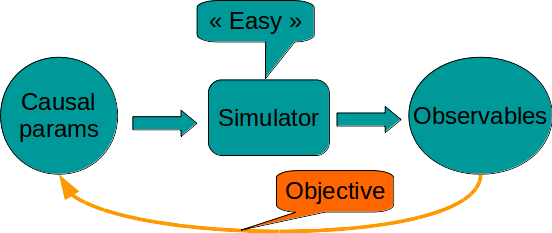
\includegraphics[width=0.8\linewidth]{inverse_problem}
    \caption{The inverse problem objective is to go from the observables to the causal parameter of the model embeded by the simulator}
    \label{fig:inverse_problem}
\end{figure}






\subsection{Hand crafted dimension reduction} % (fold)
\label{sub:hand_crafted_dimension_reduction}

\topic{Ask a theorist to build a low dimensional feature}

\content{How it was done before machine learning}


\topic{Too many dimension ? Discard the less relevants ones}

\victor{Pas sûr que ça soit vraiment utilisé. Demander à David.}






\subsection{Count estimation} % (fold)
\label{sub:count_estimation}


\topic{Classifiers can achieve optimal inference}

\content{Proof of best estimator with bayesian classifier}
\content{Intuition of classifer as separator of population in order to compute a ratio}

This section borrows many results from \cite{Neal:2007zz}.

We are studying a stochatic phenomenon which generative process is described as :

\begin{equation}
	\label{eq:mixture_model}
	p(x|m) = m p(x|S) + (1-m) p(x|B)
\end{equation}
where $x$ is the set of observable features of the studied event gathered in a vector.
Events are split into 2 classes : the signals $S$ and the backgrounds $B$.
Note that $S$ and $B$ are one of the numerous latent variable $z_i$ in \autoref{eq:intractable_integral}.
$m$ is the mixture coefficient between signals and backgrounds.

$m$ can be seen as the probability for an event to be a signal $p(S)$. 
It naturally follows that $1-m$ is the probability for an event to be a background $p(B)=1-p(S)$.
\autoref{eq:mixture_model} can be written as
\begin{equation}
	p(x) = p(S)p(x|S) + p(B)p(x|B)
\end{equation}

As previously explained the likelihoods $p(x|S)$ and $p(x|B)$ are intractable because of high dimension integrals.
However building a simulator working only in forward mode allowing to sample from $p(x|m)$ is possible.
This allow us to build a training dataset for some machine learning later.

Measurements are made from a large bunch of independant and identically distributed events $D=\{x_i\}_{i=1}^N$.

\begin{align*}
	p(D|m) =& \prod_{i=1}^N m p(x|S) + (1-m) p(x|B) \\
	       =& \prod_{i=1}^N p(x|B) \left [(1-m) + m \frac{p(x|S)}{p(x|B)} \right ]\\
	       =& \underbrace{\left[ \prod_{i=1}^N p(x|B) \right ]}_{h(x)} \times 
	       \underbrace{\left [\prod_{i=1}^N (1-m) + m \frac{p(x|S)}{p(x|B)} \right ]}_{g_m(T(x))}
\end{align*}
with $T(x) = \frac{p(x|S)}{p(x|B)} $

The Fisher-Neyman factorization theorem \needcite states that $T(x)$ is a sufficient summary statistic to obtain $m$

The maximum likelihood estimator, noted $\hat m$, is commonly used to estimate the parameter of interest.
Recall that maximum likelihood estimator are strictly equivalent to a maximum a posteriori estimator using a uniform prior.
This is a reasonable choice when we do not have prior knowledge as in this example.

\begin{equation}
	\hat m = \argmax_m p(m | D)
\end{equation}

It is more convenient (numerical stability) to express the result as a deviation from the prediction of the Standard Model.
The deviation is defined as :

\begin{equation}
	\mu = \frac{p(S)}{p_{SM}(S)} = \frac{m}{p_{SM}(S)}
\end{equation}
$p_{SM}(S)$ is the expected probability to get a signal following the Standard Model.
Recovering $m$ from $\mu$ is trivially done with $m = \mu p_{SM}(S)$.

The estimator is now :
\begin{align}
	\hmu =& \argmax_\mu p(\mu | D) \\
	     =& \argmax_\mu \frac{p(\mu)}{p(D)} p(D | \mu) \\
	     =& \argmax_\mu p(\mu) p(D | \mu) \\
	     =& \argmax_\mu  p(D | \mu) \\
	     =& \argmax_\mu  \prod_{i=1}^N g_\mu(T(x)) \\
\end{align}


$T(x)$ can be obtained using a classifier $c$ trained to separate signals and backgrounds.
A Bayes optimal classifier output gives :
\begin{equation}
	c(x) = \frac{n_s p(x|S)}{(1-n_s) p(x|B) + n_s p(x|S)}
\end{equation}
where $n_s$ is the fraction of signals used in the training dataset.

\begin{equation}
	T(x) = \frac{c(x)}{(1-c(x))} \frac{(1-s)}{s} 
\end{equation}


Note : $c$ is also a sufficient summary statistic
\begin{equation}
	g_\mu(T(x)) = 1 - \mu p_{SM}(S) + \mu p_{SM}(S) \times \frac{c(x)}{(1-c(x))} \frac{(1-s)}{s} = f_\mu(c(x))
\end{equation}

\content{Limitation : what happens if the classifier is not (Bayes) optimal ? Can we detect it ?}
\content{Physicis alos uses the Neyman-Pearson theorem on statistical test to justify maximum likelihood estimator usage. Should I include it here ? or in \autoref{sub:maximum_likelihood} ?}






\subsection{Poisson distribution} % (fold)
\label{sub:poisson_distribution}

The system allow 2 kind of collisions : soft and hard collisions.
The hard collisions are very rare compared to the soft collisions.
The data can be modeled by counting iid Bernouilli rare process which is well approximated by a Poisson distribution \needcite when the number of samples is large.
The hard collision are splitted into 2 categories the signal events and the background events.
The amount of background event $b$ is known (to a certain extent) thanks to measurement made in the data space where few or no signal can be found.

The total amout of event $n$ follows a Poisson distribution of parameter $s + b$.
Since usually $s$ is very small the parameter of interest is a deviation $\mu$ from an expected value $s$.

\begin{equation}
	n \sim Poisson(\mu s + b)
\end{equation}

Giving the likelihood :
\begin{equation}
	P(n| \mu, s, b) = \frac{(\mu s +b)^n }{n!} e^{-(\mu s + b)}
\end{equation}

A computable likelihood is now available !
This allow to use more classic parameter estimation like maximum likelihood.
The only drawback is that the nature of the event (signal/background) is not available in the data.
But a classifier can be trained to separate signals and backgrounds from training data extracted from the simulator.
As seen previously a classifier decision function is a sufficient summary statisticmaking this method optimal.
\victor{optimal method = strong claim. Better be sure about it}

To improve inference the classifier is also used to select a bunch of regions rich in signals.
\victor{(yes but how/why !!) Probably a simple result link to signal / noise ratio but I can't find it...}
Leading to a binned likelihood :

\begin{equation}
	p(D|\mu) = \prod_{i=1}^M Poisson(n_i | \mu, s_i, b_i) = \prod_{i=1}^M \frac{(\mu s_i + b_i)^n }{n!} e^{-(\mu s_i + b_i)}
\end{equation}







\subsection{Workflow} % (fold)
\label{sub:workflow}

\victor{En fait qu'est-ce que je veux dire ici ?}

In practice the data go through many processes like trigger selection, tracking, event reconstructions, etc computing hand crafted features to reduce the dimensionality from $\RR^{100 000}$ to $\RR^{40}$ then using machine learning to reduce to $\RR$.
Although machine learning is slowly taking place in some of these steps \needcite.
All the domain knowledge is concentrated in the simulator and the hand crafted data processing.


\begin{figure}[htb]
    \centering
    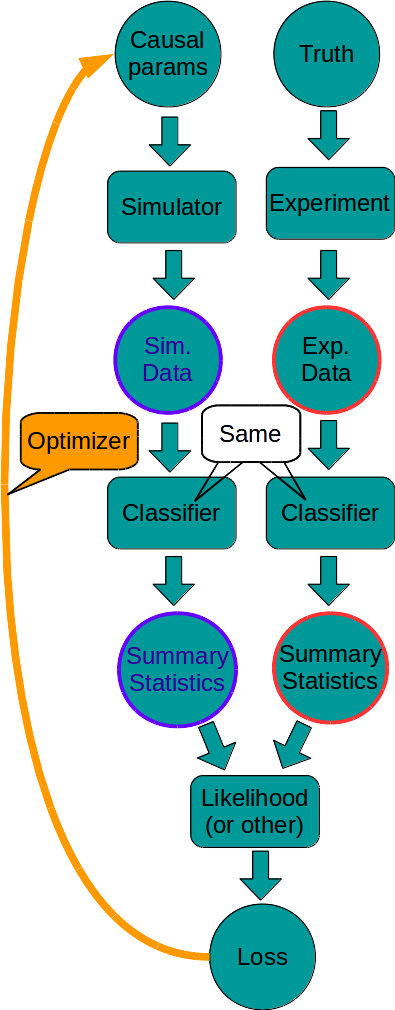
\includegraphics[width=0.3\linewidth]{workflow}
    \caption{The workflow of maximum likelihood inference using an optimizer}
    \label{fig:workflow}
\end{figure}











\section{Systematic effects} % (fold)
\label{sec:systematic_effects}

\topic{Systematic effects make inference more complex by introducing nuisance parameters}





\subsection{Definition} % (fold)
\label{sub:definition}

\content{Definition and example of systematic effects (not only in HEP !)}
\victor{Laisser le lecteur penser de lui même à l'adaptation de domaine.}

Définition de la variance :

$\VV(Y) = \EE[(Y - \EE[Y])^2] = \EE(Y^2) - [\EE(Y)]^2$

Théorème de la variance totale \needcite :

\begin{eqnarray}
    \VV[Y] =& \EE_X \left (\VV[Y|X] \right ) &+ \VV_X \left (\EE[Y|X]\right ) \\
    \VV[Y] =& \EE_X \left (\VV[Y|X] \right ) &+ \EE_X \left ( (\EE [Y|X]  - \EE[Y])^2\right )
\end{eqnarray}


En remplaçant la v.a. $Y$ par $y|x$ et $X$ par $\alpha$ on obtient :

$$
\VV[y|x] = \EE_{\alpha \sim p(\alpha|x)} \left (\VV[y|x, \alpha] \right ) + \EE_{\alpha \sim p(\alpha|x)} \left ( (\EE [y|x, \alpha]  - \EE[y|x])^2\right )
$$


On dirait presque que : 
$$\EE_{\alpha \sim p(\alpha|x)} \left ((\EE [y|x, \alpha]  - \EE[y|x])^2\right )$$
représente l'erreur systématique. 
Car c'est l'écart de notre estimation de $y$ sachant $x$ et $\alpha$ par rapport à la moyenne.
Surtout, si $\alpha|x$ est parfaitement connu (ie c'est un dirac) alors ce terme s'annule !

Mais je ne suis pas sûr que l'on puisse dire que
$$\EE_{\alpha \sim p(\alpha|x)} \left (\VV[y|x, \alpha] \right )$$
représente l'erreur statistique.

Mais si ça marche on aurrait une définition claire et précise de ce qu'est l'erreur statistique et l'erreur systématique.


\content{Schéma inverse problem with nuisance parameters}






\subsection{Classifier optimality} % (fold)
\label{sub:classifier_optimality}

\topic{Systematic effect breaks the optimality of the classifier}

\content{Why the proof does not work anymore}

\content{Poisson likelihood is not broken but weakened}


\begin{equation}
	p(D|\mu, \alpha) = \underbrace{\left[ \prod_{i=1}^N p(x|B, \alpha) \right ]}_{h_\alpha(x)} \times 
       \underbrace{\left [\prod_{i=1}^N (1-\mu) + \mu \frac{p(x|S, \alpha)}{p(x|B, \alpha)} \right ]}_{g_\mu(T_\alpha(x))}
\end{equation}



\subsection{Variance estimations} % (fold)
\label{sub:variance_estimations}

\topic{We can measure the effect of systematics on the final variance (inference is still possible)}

\content{On a caché ça sous le tapis jusqu'à maintenant mais c'est le coeur du sujet !}
\content{It does not "breaks" it but increase the variance/uncertainty}
\content{Introduce systematic vs statistical uncertainty as the 2 component of the variance}
\content{Glen's formulas ?}

\content{Marginalization could do the job but is computationally expensive}





\subsection{Profiled likelihood} % (fold)
\label{sub:profiled_likelihood}

\topic{The current way of measuring the variance of our estimation to include systematics is "profiled likelihood"}

\content{Explain how profiled likelihood works and why is works}
\content{Introduce Fisher information matrix and Cramer Rao bound (since we will use it later for INFERNO)}


references : 
\begin{itemize}
	\item \url{https://arxiv.org/abs/physics/0403059}
	\item \url{https://arxiv.org/abs/1007.1727}
\end{itemize}




\subsection{Looking for better} % (fold)
\label{sub:looking_for_better}

\topic{This document is about going further than the "simple" classifier method}

\content{Annonce de la suite / du plan du manuscrit}


